\begin{appendices}

\chapter{Terminology}
\label{appendix:terminology}

Traffic control engineering involves specific terminology to refer to different signal controls, timing plans, and controller types. This section offers a brief introduction of traffic signal control and terminology.

Modern intersections with traffic signals are controlled by a roadside \emph{signal controller}. Controllers switch power to signal lanterns and determine the sequence of display for each set of lights, operating under the safety requirement that no two conflicting flows receive green signals simultaneously. A typical controller operates lights in sequences called \emph{phases}, which are dynamic length allocations of green light time to a set of non-conflicting flows at an intersection. Typically, modern controllers include the following fixed or dynamic time allocations within a phase:

\begin{itemize}
\item \emph{late start time}, a fixed length of time a green light may be delayed for safety of other movements (e.g. pedestrian protection)
\item \emph{minimum green time}, a fixed length of time that a phase must operate before changing
\item \emph{inter-green time}, a fixed length of time required to operate amber and red signals at the end of a phase, typically at least 6 seconds. 
\item \emph{extension green time}, a dynamic length of time allocated to a phase determined after all required fixed times have been deducted from the total phase tie. 
\item \emph{maximum green time}, if the addition of the previous four time allocations exceeds the fixed maximum green time the phase is forced to change. 
\end{itemize}

A \emph{cycle} (or \emph{plan}) is an ordered sequence of one or more phases which is repeated by a controller. A fixed cycle traffic controller runs each phase for a fixed length of time within a static cycle. An actuated traffic controller can respond to sensor inputs from lane road loops and skip phases that are not in demand. Adaptive traffic controllers differ in implementation but typically can extend or shorten the length of a phase if a queue is completely cleared midway through a phase. The length of a cycle of an adaptive controller can be adapted to demand, typically running for a shorter length of time during quiet traffic and increasing in length to reduce queuing and satisfy high demand peaks \cite{scatstraining}.

An intersection has a given \emph{capacity}, defined as the maximum sustainable flow rate at which vehicles or pedestrians can travel through the intersection in a given time period. Capacity is dependant on the geometric layout of an intersection (e.g. width of road, number of lanes), driving and surface conditions, and traffic conditions. The \emph{degree of saturation} of an intersection is a ratio of arrival flow rate with respect to capacity of each approach for a given period. Arrival flow rate, also called \emph{demand flow}, refers to the number of vehicles or pedestrians arriving during a given period, measured from the back of a queue \cite{sidraglossary}. A section of road is said to be saturated if the traffic flow is equivalent to the capacity of the road at a given speed, such that any increase in flow will have a negative impact on the flow through the system. Any section of road where demanded traffic flow exceeds capacity is said to be \emph{congested} \cite{wallis2013costs}.

\chapter{Inter-Vehicle Communication}
\label{appendix:inter-vehicle-comms}

The ubiquity of mobile communication devices and modern wireless capabilities have offered new possibilities for inter-vehicle communication within road networks. Previous research suggests that short-range wireless communication devices installed in road vehicles can be used to form mobile ad-hoc networks between near proximity clusters of traffic \cite{adaptive2007grad,nadeem2004trafficview,yang2004vehicle}. Dedicated short-range communication (DSRC) is a standard for vehicle-to-vehicle and vehicle-to-infrastructure communication, currently under active development in the United States\cite{dsrc2011}.

Car-to-car communication and car-to-controller communication has been researched as a replacement for loop detection used by adaptive traffic controllers \cite{adaptive2007grad}. In this implementation, vehicles periodically transmit information about themselves and other nearby vehicles to a traffic controller using one-hop broadcasts. A traffic signal controller maintains a record of each known vehicle within range and optimises cycle length and phase timings based for the succeeding phase based on real-time information from each approach. Experimentation results suggest that adaptive traffic control using a simple traffic actuated method out-performs a predetermined phase controller by a significant factor when total intersection delay is the primary measure of effectiveness at an intersection. While these results are promising, the work is limited in scope by the use of a predetermined phase time controller as a baseline for experimentation. The increase in performance measured by the authors does not take into account the advantages of existing traffic actuated or adaptive controller schemes over an isolated, fixed-cycle controller which are likely to be significant. 

Wireless communication between vehicles and signal controllers can provide more information at an earlier stage of approach than loop detectors, including characteristics of a vehicle (number of passengers, size, weight, type of activity), speed of approach and current position. Research in this field has explored the use of vehicle-to-vehicle communication for early warning safety systems, collision avoidance, and as a means of informing vehicle passengers about road network conditions; suggesting widespread benefits for use of the technology beyond traffic modeling at controlled intersections \cite{nadeem2004trafficview,yang2004vehicle}. 

\chapter{PBTC Control Algorithm}
\label{appendix:pbtc-control}

Pseudocode for the PBTC control algorithm described in \ref{sec:PBTCDesign} is given below. The algorithm determines whether a phase change sequence is required and if so, determines the length of time the current phase duration should be extended based on estimates of the delay and stopping cost incurred by vehicles up to $K$ seconds into the future.

\begin{algorithm}[H]
 \SetAlgoLined
 \KwData{
 	$Approaches$: set of approaches, $K$: lookahead window size
 }
 \KwResult{ time in seconds before phase change should be executed or -1 for no change }
 \Begin{
  set $totalStoppingCost$ = 0 \; \\
  set $totalDelayCost$ = 0 \; \\
  \For{approach in $Approaches$}{
  	\If{approach signal is red} {
		add cost of delay for all vehicles queued on approach to $totalDelayCost$ \;
	} 
	\Else{
		add cost of stopping and cost of minimum delay for all vehicles on approach to $totalStoppingCost$ \;
	}
  }
  \If {$stoppingCost < delayCost$} {
  	set $lookaheadTable$ = [] \;
	\For{$i := 0$ to $K$} {
		$lookaheadTable$[$i$] = cost of delay for all stopped approaches over $i$ + cost of stopping for all vehicles that cannot clear the intersection within $i$ seconds \;
	}

  set $extendedGreenTime$ = index of min($lookaheadTable$) \; \\
  return $extendedGreenTime$ \;
}
return -1 \;	 \tcc*[r]{no change scheduled}
 }
 \caption{PBTC phase scheduling algorithm}
\end{algorithm}

\chapter{SCATS Data File Format}
\label{appendix:scats_data_file}

This section contains an excerpt from a data file generated by the SCATS TrafficReporter application, and provided to this project by the Wellington City Council for research purposes. The data shown represents three cycles of SCATS operation at the intersection of Victoria Street and Vivian Street in Central Wellington, between 6:00AM and 6:02AM on the 20th June, 2013. An brief explanation of the format of relevant data is given below.

\begin{verbatim}
Thursday 20-June-2013 06:00 SS   3   PL 5.3  PVa3.3 CT   65 +0 RL 65, SA 10  DS 44
 Int   SA/LK    PH  PT!  DS  VO  VK!  DS  VO  VK!  DS  VO  VK!  DS  VO  VK! ADS
  520 S  10  '   A  36!  64  10  10!  57   9  10!   -       -!   -       -!   44
  520 S  11 ^    2  26!  17   2   2!   0   0   0!   -       -!   -       -!   19
  530 S  12 *'   A  35!  57   9   8!  41   7   6!   -       -!   -       -!   35
  530 S  13      B  24!  30   4   3!  16   2   2!  15   2   2!   -       -!   14
  520 S 273 ^    B  26!  17   2   2!   -       -!   -       -!   -       -!   23
A=<65>  B=35
Thursday 20-June-2013 06:01 SS   3   PL 5.3  PVa2.3 CT   65 +0 RL 65, SA 10  DS 54
 Int   SA/LK    PH  PT!  DS  VO  VK!  DS  VO  VK!  DS  VO  VK!  DS  VO  VK! ADS
  520 S  10  '   A  41!  43   8   7!  55  11  11!   -       -!   -       -!   54
  520 S  11 ^    2  25!  14   2   2!  56   4   6!   -       -!   -       -!   36
  530 S  12 *'   A  67!  26   8   7!  36  11  10!   -       -!   -       -!   40
  530 S  13      B   0!   0   0   0!   0   0   0!   0   0   0!   -       -!   10
  520 S 273 ^    B  25!   0   0   0!   -       -!   -       -!   -       -!   13
A=<64>  B=36
Thursday 20-June-2013 06:02 SS   3   PL 5.3  PV 0.3 CT   65 +0 RL 65, SA 10  DS 44
 Int   SA/LK    PH  PT!  DS  VO  VK!  DS  VO  VK!  DS  VO  VK!  DS  VO  VK! ADS
  520 S  10  '   A  65!  27   9   7!  21   8   6!   -       -!   -       -!   44
  520 S  11 ^    2   0!   0   0   0!   0   0   0!   -       -!   -       -!   22
  530 S  12 *'   A  41!  12   3   2!  34   7   6!   -       -!   -       -!   40
  530 S  13      B  23!  11   2   1!   0   0   0!   0   0   0!   -       -!   12
  520 S 273 ^    B   0!   0   0   0!   -       -!   -       -!   -       -!    4
A=<64>  B=36
\end{verbatim}

\begin{itemize}
\item \textbf{Int} Intersection, the unique identifier of the intersection each data line corresponds to. Some log files can include data from nearby intersections to help traffic engineers report on an entire subsystem. The snippet above shows data for intersections 520 and 530.
\item \textbf{SA/LK} Strategic Approach/Link, the identifier to describe an approaching road, unique within an intersection.
\item \textbf{PH} Phase, the alphabetical character identifier used to name the phase that was operated. Typically the letters A-F are used to describe each phase. 
\item \textbf{PT!} Phase time, the duration in seconds of the phase that was operated.
\item \textbf{DS} Degree of Saturation, the degree of saturation measured for traffic flow during the cycle.
\item \textbf{VO} Vehicle actuations, the number of vehicles that were counted by stop-line detectors during the cycle.
\end{itemize}

\chapter{Evaluation Intersections}
\label{appendix:scats_intersections}

Three intersections within the Wellington City central road network were selected as the basis for evaluation of this project. Figure ~\ref{intersectionmap} shows a map of Wellington City, marked with the location of the three intersections considered, Vivian Street and Victoria Street, Courtenay Place and Tory Street, and Karo Drive and Victoria Street. The intersections were selected based on the availability of logged data from the Wellington City Council, capability of the PBTSim simulator to model the intersections appropriately, and variations in traffic volume to investigate the performance of the PBTC control algorithm in multiple realistic traffic scenarios. The map shown was generated using Google Maps \cite{googlemaps}.

\begin{figure}[]
\centering
	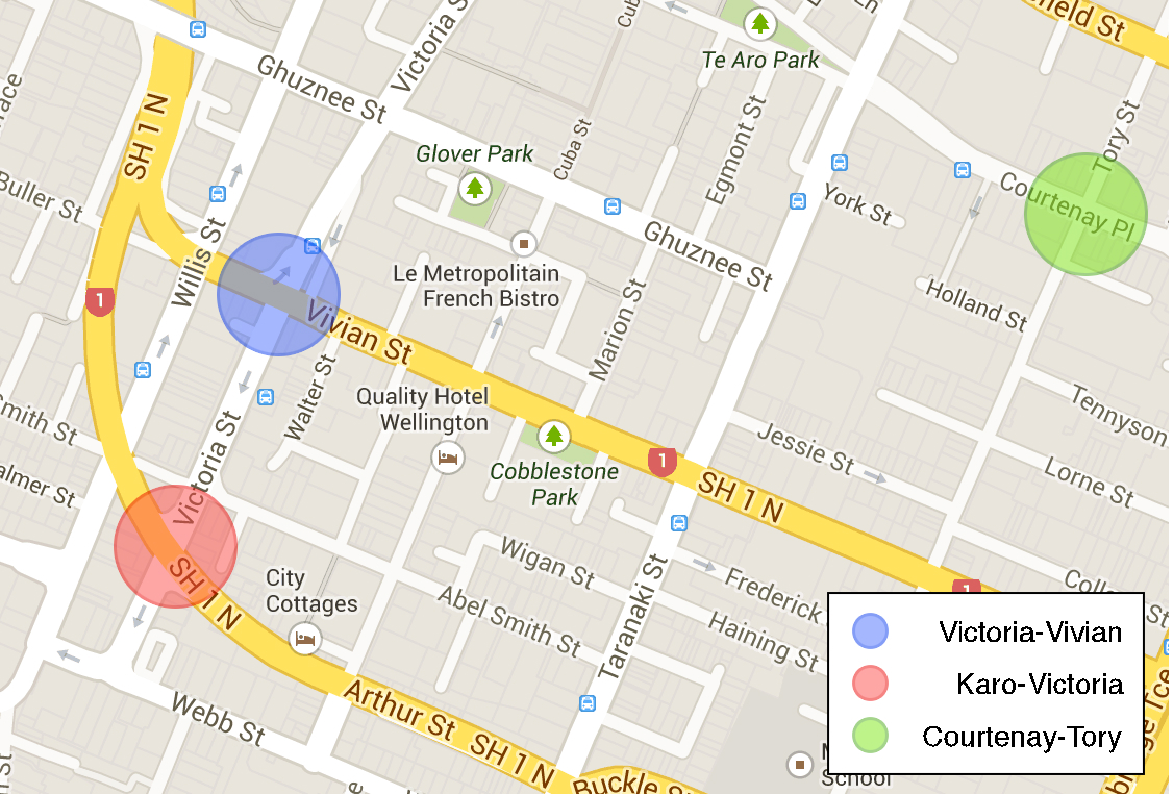
\includegraphics[scale=0.5]{intersection-map.pdf}
	\caption[A map of Wellington City showing intersections used for evaluation]{ A map of Wellington City showing the intersections of Vivian Street and Victoria Street, Courtenay Place and Tory Street, and Karo Drive and Victoria Street marked. }
\label{intersectionmap}
\end{figure}


\section{SCATS Representations} 

Figure ~\ref{scats_intersections} shows the three evaluation intersections used during evaluation of the PBTC system as represented in the SCATS system used by Wellington City Council. Screenshots were provided by Wellington City Council traffic engineers. The SCATS phase configuration for each intersection is shown to the left of each figure. Note that in the case of Courtenay-Tory, phases A, B, C, E, E1, and E2 are considered as a single phase in the SCATS log files and PBTSim configuration.


\begin{figure}[]
\centering
\begin{subfigure}{.5\textwidth}
  \centering
  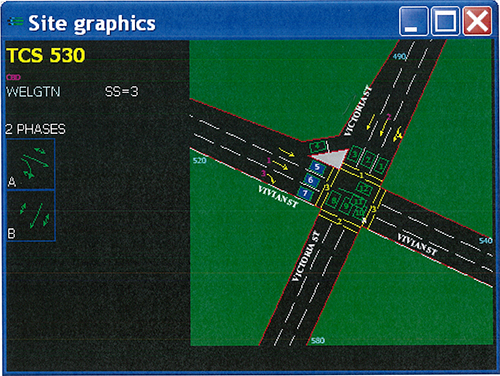
\includegraphics[scale=0.35]{scats-vivian-victoria.png}
  \caption{Vivian Street-Victoria Street}
  \label{fig:sub1}
\end{subfigure}%
\begin{subfigure}{.5\textwidth}
  \centering
  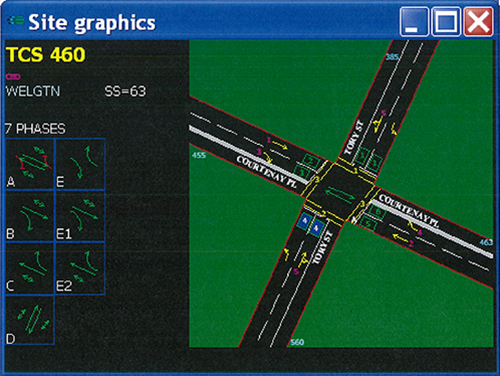
\includegraphics[scale=0.35]{scats-courtenay-tory.png}
  \caption{Courtenay Place-Tory Street}
  \label{fig:sub2}
\end{subfigure}

\vspace{1cm}

\begin{subfigure}{.5\textwidth}
  \centering
  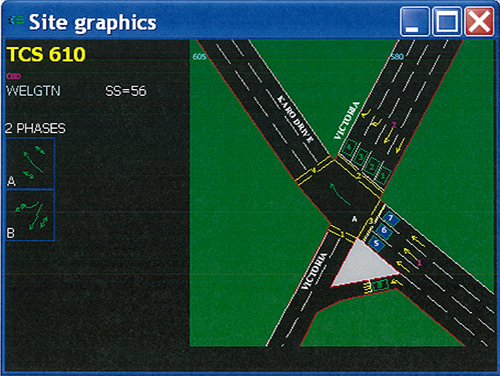
\includegraphics[scale=0.35]{scats-karo-victoria.png}
  \caption{Karo-Victoria}
  \label{fig:sub1}
\end{subfigure}%
\caption{ Screenshots of the Vivian-Victoria, Courtenay-Tory, and Karo-Victoria intersections as represented in the SCATS system. }
\label{scats_intersections}
\end{figure}

\section{PBTSim Representations}

Figure ~\ref{pbtsim_intersections} shows the visual representation of the three evaluation intersections within the PBTSim graphical user interface. All lanes catering for turning traffic have been omitted from each intersection and are not considered by this project. 

\begin{figure}[]
\centering
\begin{subfigure}{.5\textwidth}
  \centering
  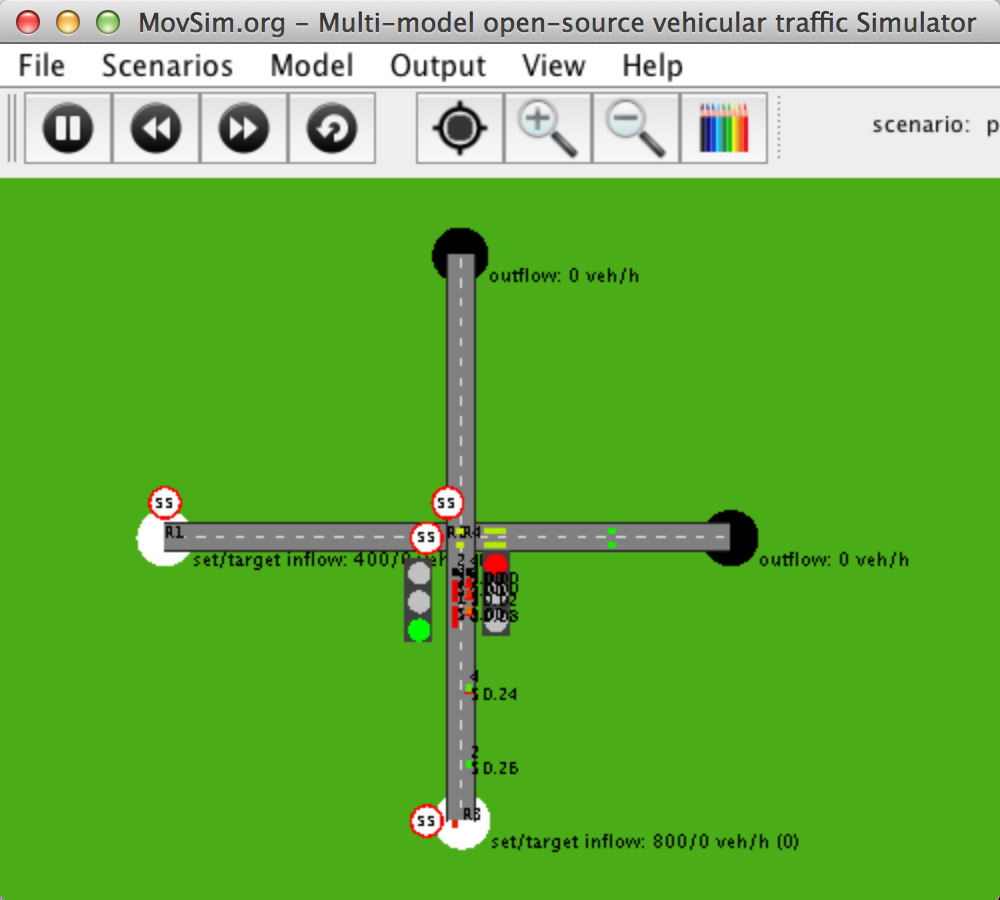
\includegraphics[scale=0.35]{pbtsim-vivian-victoria.png}
  \caption{Vivian-Victoria}
  \label{fig:sub1}
\end{subfigure}%
\begin{subfigure}{.5\textwidth}
  \centering
  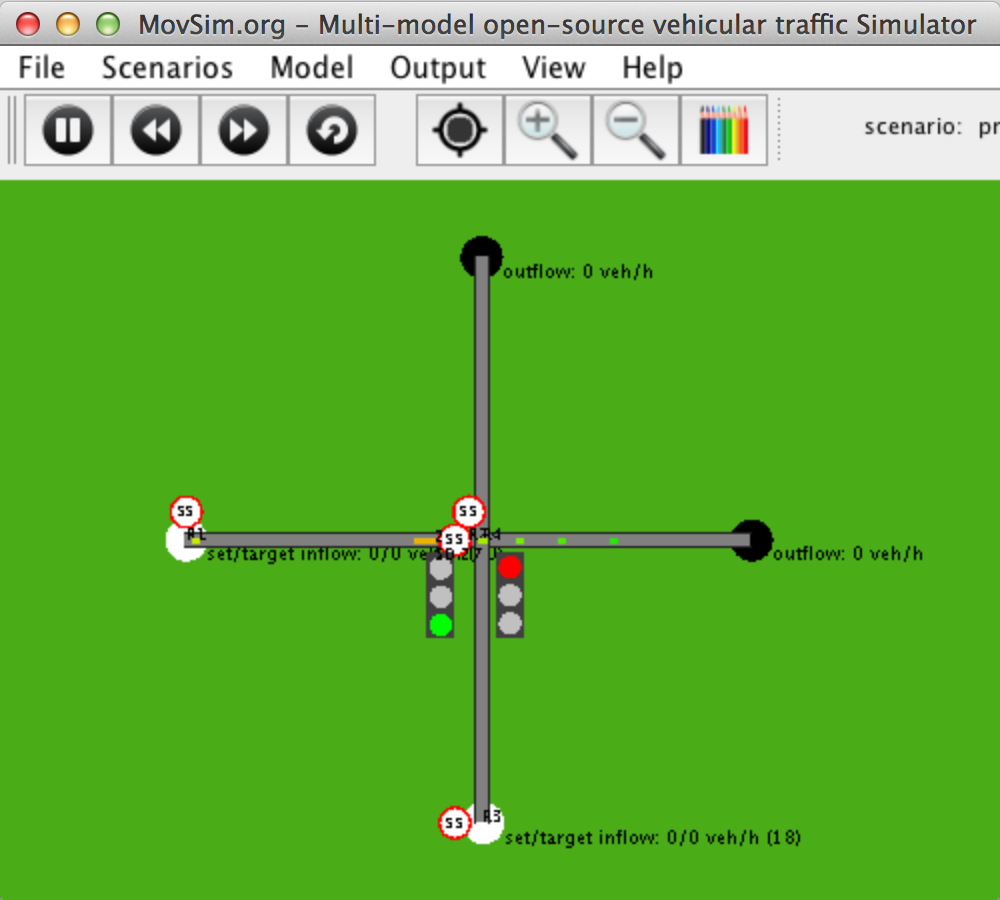
\includegraphics[scale=0.35]{pbtsim-courtenay-tory.png}
  \caption{Courtenay-Tory}
  \label{fig:sub2}
\end{subfigure}

\vspace{1cm}

\begin{subfigure}{.5\textwidth}
  \centering
  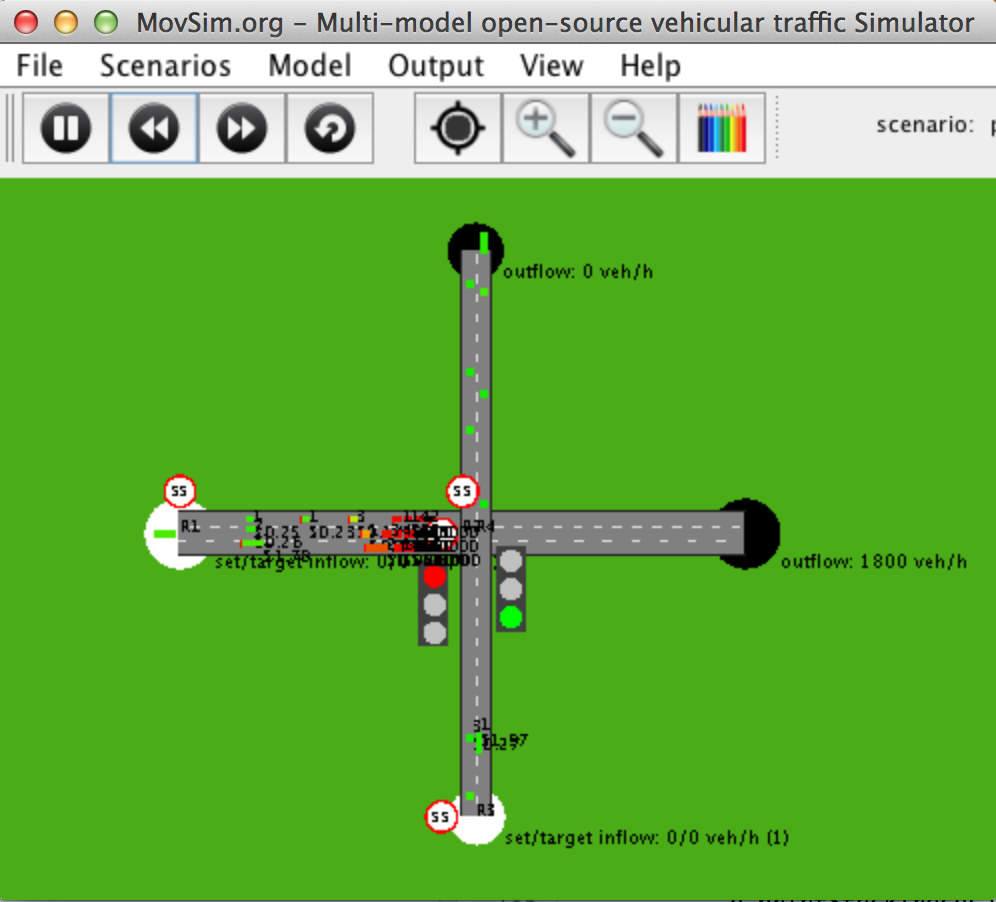
\includegraphics[scale=0.35]{pbtsim-karo-victoria.png}
  \caption{Karo-Victoria}
  \label{fig:sub1}
\end{subfigure}%
\caption[Screenshows of the Vivian-Victoria, Courtenay-Tory, and Karo-Victoria intersections as represented in the PBTSim simulator.]{ Intersections of Vivian-Victoria, Courtenay-Tory, and Karo-Victoria as represented in the PBTSim simulator.  }
\label{pbtsim_intersections}
\end{figure}

\end{appendices}
